\documentclass{standalone}
\usepackage{tikz}
\begin{document}
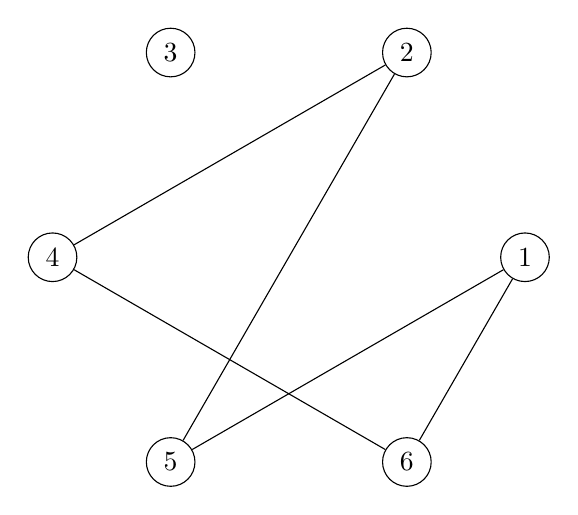
\begin{tikzpicture}[scale=1, every node/.style={circle, draw}]
\node (N1) at (3.00,0.00) {1};
\node (N2) at (1.50,2.60) {2};
\node (N3) at (-1.50,2.60) {3};
\node (N4) at (-3.00,0.00) {4};
\node (N5) at (-1.50,-2.60) {5};
\node (N6) at (1.50,-2.60) {6};
\draw (N1) -- (N5);
\draw (N1) -- (N6);
\draw (N2) -- (N4);
\draw (N2) -- (N5);
\draw (N4) -- (N6);
\end{tikzpicture}
\end{document}
